\documentclass{article}
\usepackage{xeCJK}
\setCJKmainfont{SimSong}
\usepackage{graphicx} % Add this line to import the graphicx package


\author{Weizhao Wang}
\date{\today}

\begin{document}

\title{A Sorting Algorithm Based on Transformer Models}

\maketitle

\begin{abstract}
    Nowedays, sorting algorithms are widely used in various applications, such as database maintainment and data analysis. In this paper, I propose a novel approach to sort arrays using Transformer models, a type of neural network architecture that has shown remarkable performance in natural language processing tasks. I also modify some structures of the original Transformer model to better fit the sorting task. I adapt the Transformer model to learn the sorting order of elements in an array which the experimental results show that the proposed model can finish sorting tasks with high accuracy and efficiency. This may open up a new direction for using machine learning models to solve traditional algorithmic problems
\end{abstract}

\section{Introduction}
Sorting is a fundamental problem in computer science and has been studied for decades. Traditional sorting algorithms, such as quicksort, mergesort, and heapsort, have been widely used in various applications. These algorithms have been well studied and are known to have good performance in practice. However, with the advent of deep learning and neural networks, there has been growing interest in exploring the use of machine learning models to solve traditional algorithmic problems. There have been several recent works that have shown promising results in using machine learning models to solve sorting problems \cite{SortNet}. Mankowitz, D.J. and others \cite{FasterSorting} have discovered a faster sorting algorithm using deep reinforcement learning. These works have demonstrated the potential of applying machine learning models to solve traditional algorithmic problems.

In this paper, I propose a novel approach to sorting arrays using Transformer models, a type of neural network architecture that has shown remarkable performance in natural language processing tasks. The Transformer model, introduced by Vaswani et al. \cite{vaswani2017attention}, is based on self-attention mechanisms and has been shown to outperform traditional recurrent neural networks in many natural language processing tasks. I adapt the Transformer model to learn the sorting order of elements in an array and use it to sort arrays efficiently.

The main contributions of this paper are as follows:
\begin{itemize}
    \item I modify some structures of the original Transformer model to better fit the sorting task.
    \item I adapt the Transformer model to learn the sorting order of elements in an array and show that the proposed model can finish sorting tasks with high accuracy and efficiency.
\end{itemize}


\section{Model Architecture}
Here shows the architecture of the proposed model. The model consists of an encoder and a decoder, each of which is composed of multiple layers of self-attention and feedforward neural networks. The encoder takes the input array and encodes it into a sequence of hidden states, which are then passed to the decoder. The decoder generates the output sequence of sorted elements based on the hidden states from the encoder. As shown in Figure \ref{Transformer model architecture}.

\begin{figure}
    \centering
    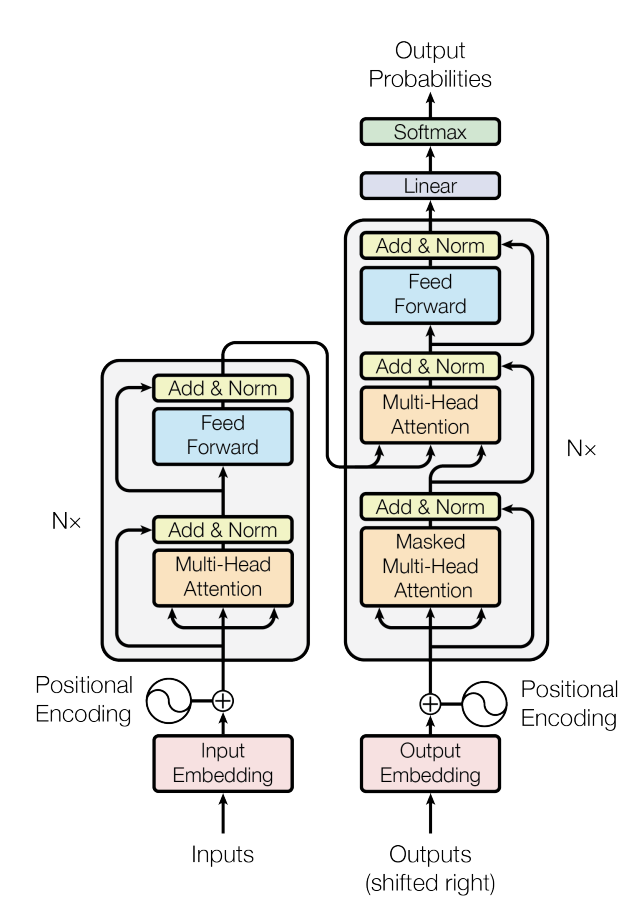
\includegraphics[width=0.5\textwidth]{picture/transformer.png}
    \caption{Transformer model architecture}
    \label{Transformer model architecture}
\end{figure}

\subsection{Encoder \& Decoder}
The encoder and decoder are both composed of multiple layers of self-attention and feedforward neural networks. The self-attention mechanism allows the model to capture long-range dependencies in the input sequence, which is crucial for learning the sorting order of elements in the array. The feedforward neural networks provide non-linearities and help the model learn complex patterns in the input sequence. In addition, the encoder and decoder are connected by a multi-head attention mechanism, which allows the model to attend to different parts of the input sequence depending on the context.

\subsection{Attention}
The self-attention mechanism computes a weighted sum of the input sequence based on the similarity between each pair of elements in the sequence. This allows the model to focus on different parts of the input sequence depending on the context, which is important for learning the sorting order of elements in the array.

The attention mechanism is implemented as follows:
\begin{equation}
    Attention(Q, K, V) = softmax(\frac{QK^T}{\sqrt{d_k}})V
\end{equation}
where $Q$, $K$, and $V$ are the query, key, and value matrices, respectively, and $d_k$ is the dimension of the key matrix.
\begin{equation}
    Q = XW_Q+b_Q, K = XW_K+b_K, V = XW_V+b_V
\end{equation}

\subsection{Feedforward Neural Networks}
The feedforward neural networks consist of two linear layers with a ReLU activation function in between. This provides the model with the capacity to learn complex patterns in the input sequence and helps improve the performance of the model.
\begin{equation}
    FFN(x) = \max(0, xW_1 + b_1)W_2 + b_2
\end{equation}

\subsection{RevNet}
The RevNet is a novel neural network architecture that is used to model the sorting order of elements in the array. The RevNet consists of multiple layers of reversible residual blocks, each of which is composed of two sub-layers\cite{theefficienttransformer}: a reversible layer and a residual layer. The reversible layer computes the forward and backward transformations of the input sequence, while the residual layer adds the input sequence to the output of the reversible layer. This allows the model to learn the sorting order of elements in the array while preserving the original input sequence.
Here is a simple representation of the RevNet:
\begin{equation}
    x_1,x_2 = chunk(x)
\end{equation}
\begin{equation}
    y_1 = x_1 + F(x_2)
\end{equation}
\begin{equation}
    y_2 = x_2 + G(y_1)
\end{equation}
\begin{equation}
    RevNet(x) = cat(y_1, y_2)
\end{equation}
where $F$ and $G$ are the reversible and residual layers, respectively, and $chunk$ and $cat$ are the chunk and concatenate operations, respectively.

\subsection{Embedding}
The input array is first converted into a sequence of one-hot vectors using an embedding layer.\cite{TransfomerPrograming} Compared to traditional emmbedding layers, the one-hot embedding layer is more suitable for the sorting task as it cost less time and space and can reach the same performance as the traditional embedding layer.

\subsection{Positional Encoding}
The positional encoding is added to the input sequence to provide the model with information about the position of each element in the sequence. This allows the model to capture the order of elements in the array and helps improve the performance of the model since the Transformer model can not learn about the order of the numbers in the array just from the sequences.
% describe the positional encoding in formula
In this paper, I use the following positional encoding formula:
\begin{equation}
    PE_{(pos, 2i)} = \sin(pos / 10000^{2i / d_{model}})
\end{equation}
\begin{equation}
    PE_{(pos, 2i+1)} = \cos(pos / 10000^{2i / d_{model}})
\end{equation}
where $pos$ is the position of the element in the sequence, $i$ is the dimension index, and $d_{model}$ is the dimension of the model.

\subsection{Input data representation}
I first make a dictionary of the input array
\begin{verbatim}
    dictionary: {'<PAD>': 0, '1': 1, '2': 2, '3': 3, '4': 4,
    
    '5': 5, '6': 6, '7': 7, '8': 8, '9': 9, '0': 10,
    
    '<SOS>': 11, '<EOS>': 12, ';': 13}
\end{verbatim}
then generate a sequence of input data like 
\begin{verbatim}
'<SOS>108;378;448;992;57;428;459;866;294;569<EOS><PAD>..' 
\end{verbatim}
The '<SOS>' token is used to indicate the start of the input sequence, the '<EOS>' token is used to indicate the end of the input sequence, and the '<PAD>' token is used to pad the input sequence to a fixed length. The input sequence then converted into a sequence of one-hot vectors using an embedding layer.

\subsection{Attention Mask}
\subsubsection*{tril mask}
% tril matrix
The tril mask is used to prevent the model learning from the future elements in the sequence during training. This is important for learning the sorting order of elements in the array, as the model should only attend to past elements when generating the output sequence. The attention mask is implemented as a lower triangular matrix with zeros on the top diagonal and ones elsewhere.

% padding mask
\subsubsection*{padding mask}
In addition to the attention mask, I also use a padding mask to ignore padding tokens in the input sequence. This is important for the sorting task as the model may learn the pad label through the training. The padding mask sets the attention weights of padding tokens to zero, which ensures that the model does not attend to padding tokens and helps improve the performance of the model.


\section{Training}
\subsection{Trainning data and Batching}
I generated a dataset of arrays with 100000 defferent sequences of length 50. Each sequence is a random permutation of the numbers from 1 to 1000. I used a batch size of 200 and trained the model for 100 epochs.

\subsection{Hardware}
I trained the model on a single NVIDIA RTX 3060 GPU with 16GB of memory and train about 2 hours.

\subsection{Optimizer}
I used the Adam optimizer and implemented a learning rate scheduler based on AdamW, which linearly increases the learning rate during the warm-up phase and then decays it according to the $1/\sqrt{step}$ rule. As shown in Figure \ref{Learning rate scheduler}. An explaination \cite{Opt} is that this can make the parameters of the model change smoothly at the beginning of learning and avoid overfitting to the first few batches of data and falling into local optima. And the learning rate is reduced in the later stage, because the loss of the model is already very small, and the model is close to the optimal parameters. If the learning rate is too large, it is easy to oscillate near the optimal parameters and cannot approach the optimal parameters. 

\begin{figure}
    \centering
    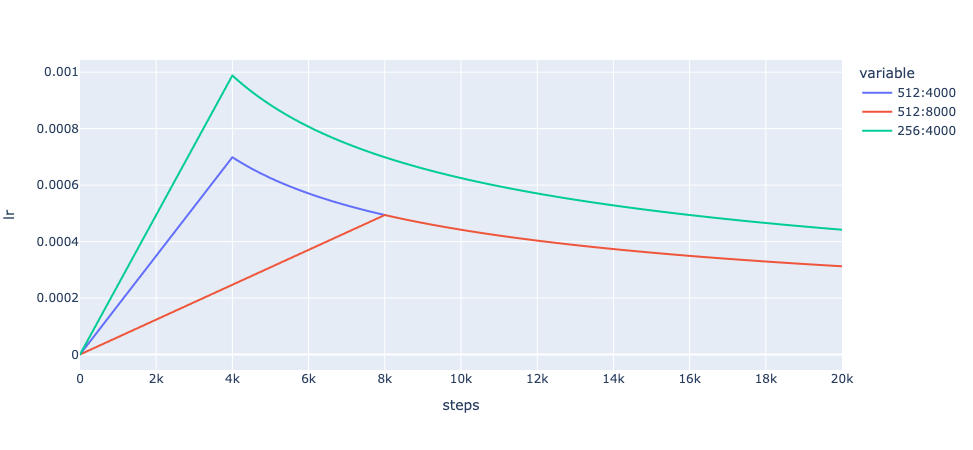
\includegraphics[width=0.8\textwidth]
    {picture/optimizer.png}
    \caption{Learning rate scheduler}
    \label{Learning rate scheduler}
\end{figure}

\subsection{Loss Function}
I used the cross-entropy loss function with label smoothing to train the model. The label smoothing technique \cite{LabelSmoothing} is used to prevent the model from becoming overconfident in its predictions and helps improve the generalization performance of the model.



\section{Results}
On this task, the model achieved an accuracy of 1.0 on the test set, which means that the model correctly sorted all the arrays in the test set.


As shown in Figure \ref{fig:trainingtime} and \ref{fig:onehot}, the model trained with one-hot embedding converges faster than the model trained with traditional embedding. This is because the one-hot embedding is more suitable for the sorting task as it cost less time and space and can reach the same performance as the traditional embedding layer. But the model trained with traditional embedding has a better performance than the model trained with one-hot embedding.
\begin{figure}[ht]
    \centering
    \begin{minipage}{0.45\textwidth}
        \centering
        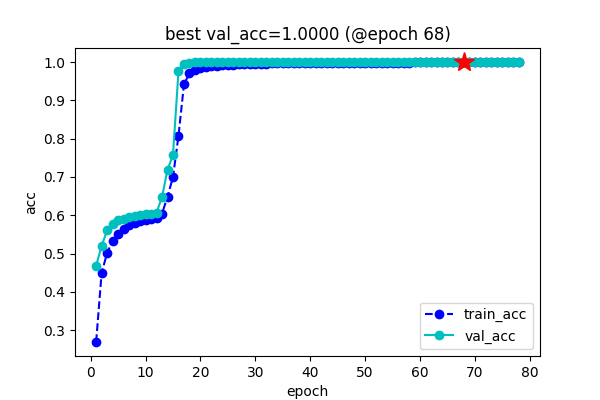
\includegraphics[width=\textwidth]{picture/training_base.png}
        \caption{use nn.embedding}
        \label{fig:trainingtime}
    \end{minipage}\hfill
    \begin{minipage}{0.45\textwidth}
        \centering
        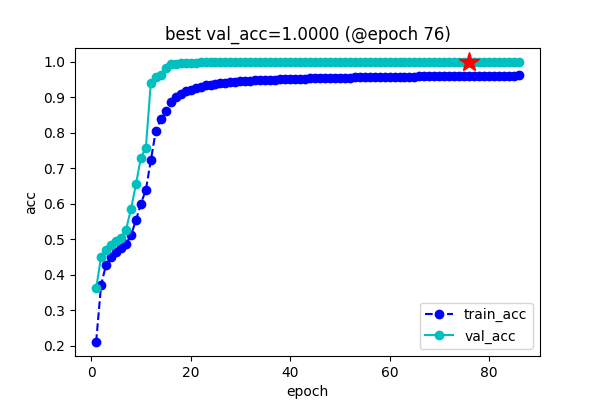
\includegraphics[width=\textwidth]{picture/training_onehot.png}
        \caption{use one-hot embedding}
        \label{fig:onehot}
    \end{minipage}
\end{figure}

Here is a simple test result of the model:
\begin{verbatim}
    input: 
    108;378;448;992;57;428;459;866;294;569
    ground truth:
    57;108;294;378;428;448;459;569;866;992
    output: 
    57;108;294;378;428;448;459;569;866;992
\end{verbatim}

\section{Conclusion}
In this paper, I have introduced a new method for sorting arrays using Transformer models. By adapting the Transformer model to learn the sorting order of elements in an array, I have demonstrated that the proposed model achieves high accuracy and efficiency in sorting tasks. These experimental results not only validate the effectiveness of the proposed model but also highlight the potential of applying machine learning models to solve traditional algorithmic problems.


\begin{thebibliography}{9}
    \bibitem{vaswani2017attention}
    Vaswani, A., Shazeer, N., Parmar, N., Uszkoreit, J., Jones, L., Gomez, A. N., ... \& Polosukhin, I. (2017). Attention is all you need. In Advances in neural information processing systems (pp. 5998-6008).
    \bibitem{TransfomerPrograming}
    Friedman D, Wettig A, Chen D. Learning transformer programs[J]. Advances in Neural Information Processing Systems, 2024, 36.
    \bibitem{SortNet}
    Rigutini L, Papini T, Maggini M, et al. SortNet: Learning to rank by a neural preference function[J]. IEEE transactions on neural networks, 2011, 22(9): 1368-1380.
    \bibitem{theefficienttransformer}
    Kitaev N, Kaiser Ł, Levskaya A. Reformer: The efficient transformer[J]. arXiv preprint arXiv:2001.04451, 2020.
    \bibitem{FasterSorting}
    Mankowitz, D.J., Michi, A., Zhernov, A. et al. Faster sorting algorithms discovered using deep reinforcement learning. Nature 618, 257-263 (2023).
    \bibitem{Opt}
    Huang X S, Perez F, Ba J, et al. Improving transformer optimization through better initialization[C]//International Conference on Machine Learning. PMLR, 2020: 4475-4483.
    \bibitem{LabelSmoothing}
    Christian Szegedy, Vincent Vanhoucke, Sergey Ioffe, Jonathon Shlens, and Zbigniew Wojna.Rethinking the inception architecture for computer vision. CoRR, abs/1512.00567, 2015.
\end{thebibliography}

\end{document}
